\documentclass{standalone}
\usepackage{tikz}
\usetikzlibrary{patterns, positioning}

\begin{document}
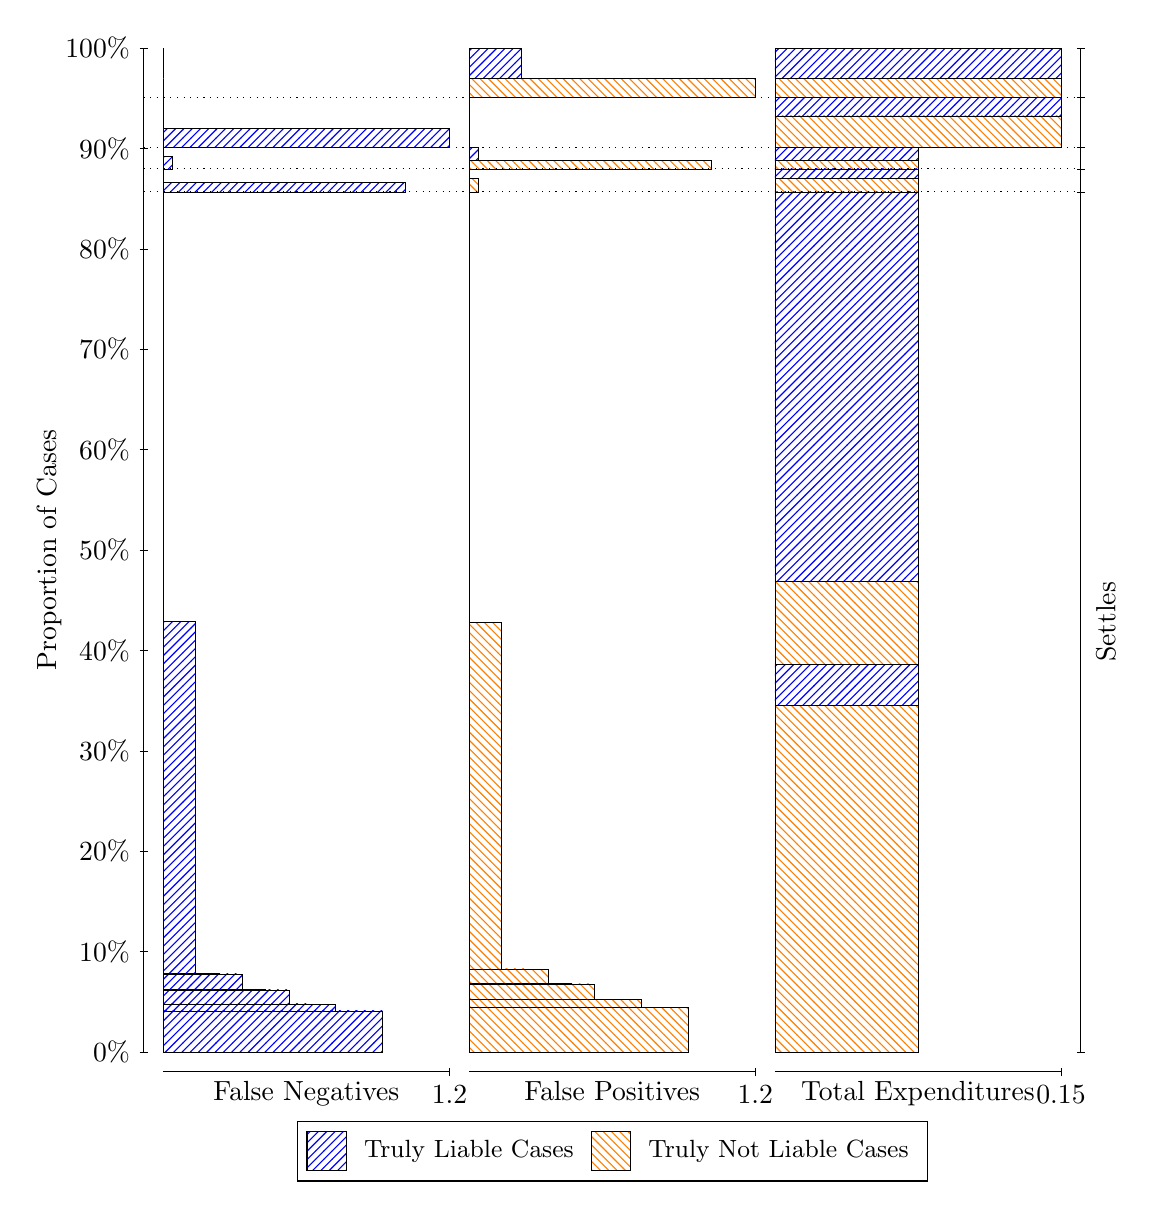
\begin{tikzpicture}
\draw[black, very thin] (1.5,1.75) -- (1.5,14.5);
\node[rotate=90, anchor=center] at (0.3, 8.125) {Proportion of Cases};
\draw[black, very thin] (1.45,1.75) -- (1.55,1.75);
\node[anchor=east] at (1.45, 1.75) {0\%};
\draw[black, very thin] (1.45,3.025) -- (1.55,3.025);
\node[anchor=east] at (1.45, 3.025) {10\%};
\draw[black, very thin] (1.45,4.3) -- (1.55,4.3);
\node[anchor=east] at (1.45, 4.3) {20\%};
\draw[black, very thin] (1.45,5.575) -- (1.55,5.575);
\node[anchor=east] at (1.45, 5.575) {30\%};
\draw[black, very thin] (1.45,6.85) -- (1.55,6.85);
\node[anchor=east] at (1.45, 6.85) {40\%};
\draw[black, very thin] (1.45,8.125) -- (1.55,8.125);
\node[anchor=east] at (1.45, 8.125) {50\%};
\draw[black, very thin] (1.45,9.4) -- (1.55,9.4);
\node[anchor=east] at (1.45, 9.4) {60\%};
\draw[black, very thin] (1.45,10.675) -- (1.55,10.675);
\node[anchor=east] at (1.45, 10.675) {70\%};
\draw[black, very thin] (1.45,11.95) -- (1.55,11.95);
\node[anchor=east] at (1.45, 11.95) {80\%};
\draw[black, very thin] (1.45,13.225) -- (1.55,13.225);
\node[anchor=east] at (1.45, 13.225) {90\%};
\draw[black, very thin] (1.45,14.5) -- (1.55,14.5);
\node[anchor=east] at (1.45, 14.5) {100\%};

\draw[black, very thin] (13.4,1.75) -- (13.4,14.5);
\draw[black, very thin] (13.35,1.75) -- (13.45,1.75);
\node[anchor=west] at (13.35, 1.75) {};
\draw[black, very thin] (13.35,12.674) -- (13.45,12.674);
\node[anchor=west] at (13.35, 12.674) {};
\draw[black, very thin] (13.35,12.966) -- (13.45,12.966);
\node[anchor=west] at (13.35, 12.966) {};
\draw[black, very thin] (13.35,13.238) -- (13.45,13.238);
\node[anchor=west] at (13.35, 13.238) {};
\draw[black, very thin] (13.35,13.876) -- (13.45,13.876);
\node[anchor=west] at (13.35, 13.876) {};
\draw[black, very thin] (13.35,14.5) -- (13.45,14.5);
\node[anchor=west] at (13.35, 14.5) {};

\draw[black, very thin, pattern color=blue, pattern=north east lines] (1.75,1.75) rectangle (4.5306,2.2705);
\draw[black, very thin, pattern color=blue, pattern=north east lines] (1.75,2.2705) rectangle (4.234,2.2716);
\draw[black, very thin, pattern color=blue, pattern=north east lines] (1.75,2.2716) rectangle (3.9374,2.3587);
\draw[black, very thin, pattern color=blue, pattern=north east lines] (1.75,2.3587) rectangle (3.6408,2.3607);
\draw[black, very thin, pattern color=blue, pattern=north east lines] (1.75,2.3607) rectangle (3.3442,2.5391);
\draw[black, very thin, pattern color=blue, pattern=north east lines] (1.75,2.5391) rectangle (3.0476,2.542);
\draw[black, very thin, pattern color=blue, pattern=north east lines] (1.75,2.542) rectangle (2.751,2.743);
\draw[black, very thin, pattern color=blue, pattern=north east lines] (1.75,2.743) rectangle (2.4544,2.7447);
\draw[black, very thin, pattern color=blue, pattern=north east lines] (1.75,2.7447) rectangle (2.1578,7.2194);
\draw[black, very thin, pattern color=orange, pattern=north west lines] (1.75,7.2194) rectangle (1.75,12.674);
\draw[black, very thin, pattern color=blue, pattern=north east lines] (1.75,12.674) rectangle (4.8272,12.792);
\draw[black, very thin, pattern color=orange, pattern=north west lines] (1.75,12.792) rectangle (1.75,12.966);
\draw[black, very thin, pattern color=blue, pattern=north east lines] (1.75,12.966) rectangle (1.8612,13.128);
\draw[black, very thin, pattern color=orange, pattern=north west lines] (1.75,13.128) rectangle (1.75,13.238);
\draw[black, very thin, pattern color=blue, pattern=north east lines] (1.75,13.238) rectangle (5.3833,13.476);
\draw[black, very thin, pattern color=orange, pattern=north west lines] (1.75,13.476) rectangle (1.75,13.876);
\draw[black, very thin, pattern color=orange, pattern=north west lines] (1.75,13.876) rectangle (1.75,14.111);
\draw[black, very thin, pattern color=blue, pattern=north east lines] (1.75,14.111) rectangle (1.75,14.5);
\draw[black, very thin, pattern color=orange, pattern=north west lines] (5.6333,1.75) rectangle (8.4139,2.3151);
\draw[black, very thin, pattern color=orange, pattern=north west lines] (5.6333,2.3151) rectangle (8.1173,2.316);
\draw[black, very thin, pattern color=orange, pattern=north west lines] (5.6333,2.316) rectangle (7.8207,2.4191);
\draw[black, very thin, pattern color=orange, pattern=north west lines] (5.6333,2.4191) rectangle (7.5241,2.4212);
\draw[black, very thin, pattern color=orange, pattern=north west lines] (5.6333,2.4212) rectangle (7.2276,2.6141);
\draw[black, very thin, pattern color=orange, pattern=north west lines] (5.6333,2.6141) rectangle (6.931,2.6151);
\draw[black, very thin, pattern color=orange, pattern=north west lines] (5.6333,2.6151) rectangle (6.931,2.6172);
\draw[black, very thin, pattern color=orange, pattern=north west lines] (5.6333,2.6172) rectangle (6.6344,2.8032);
\draw[black, very thin, pattern color=orange, pattern=north west lines] (5.6333,2.8032) rectangle (6.3378,2.8055);
\draw[black, very thin, pattern color=orange, pattern=north west lines] (5.6333,2.8055) rectangle (6.0412,7.2048);
\draw[black, very thin, pattern color=blue, pattern=north east lines] (5.6333,7.2048) rectangle (5.6333,12.674);
\draw[black, very thin, pattern color=orange, pattern=north west lines] (5.6333,12.674) rectangle (5.7446,12.849);
\draw[black, very thin, pattern color=blue, pattern=north east lines] (5.6333,12.849) rectangle (5.6333,12.966);
\draw[black, very thin, pattern color=orange, pattern=north west lines] (5.6333,12.966) rectangle (8.7105,13.077);
\draw[black, very thin, pattern color=blue, pattern=north east lines] (5.6333,13.077) rectangle (5.7446,13.238);
\draw[black, very thin, pattern color=orange, pattern=north west lines] (5.6333,13.238) rectangle (5.6333,13.638);
\draw[black, very thin, pattern color=blue, pattern=north east lines] (5.6333,13.638) rectangle (5.6333,13.876);
\draw[black, very thin, pattern color=orange, pattern=north west lines] (5.6333,13.876) rectangle (9.2667,14.111);
\draw[black, very thin, pattern color=blue, pattern=north east lines] (5.6333,14.111) rectangle (6.3007,14.5);
\draw[black, very thin, pattern color=orange, pattern=north west lines] (9.5167,1.75) rectangle (11.333,6.1516);
\draw[black, very thin, pattern color=blue, pattern=north east lines] (9.5167,6.1516) rectangle (11.333,6.6732);
\draw[black, very thin, pattern color=orange, pattern=north west lines] (9.5167,6.6732) rectangle (11.333,7.7264);
\draw[black, very thin, pattern color=blue, pattern=north east lines] (9.5167,7.7264) rectangle (11.333,12.674);
\draw[black, very thin, pattern color=orange, pattern=north west lines] (9.5167,12.674) rectangle (11.333,12.849);
\draw[black, very thin, pattern color=blue, pattern=north east lines] (9.5167,12.849) rectangle (11.333,12.966);
\draw[black, very thin, pattern color=orange, pattern=north west lines] (9.5167,12.966) rectangle (11.333,13.077);
\draw[black, very thin, pattern color=blue, pattern=north east lines] (9.5167,13.077) rectangle (11.333,13.238);
\draw[black, very thin, pattern color=orange, pattern=north west lines] (9.5167,13.238) rectangle (13.15,13.638);
\draw[black, very thin, pattern color=blue, pattern=north east lines] (9.5167,13.638) rectangle (13.15,13.876);
\draw[black, very thin, pattern color=orange, pattern=north west lines] (9.5167,13.876) rectangle (13.15,14.111);
\draw[black, very thin, pattern color=blue, pattern=north east lines] (9.5167,14.111) rectangle (13.15,14.5);
\draw[black, dotted] (1.5,12.674) -- (13.4,12.674);
\draw[black, dotted] (1.5,12.966) -- (13.4,12.966);
\draw[black, dotted] (1.5,13.238) -- (13.4,13.238);
\draw[black, dotted] (1.5,13.876) -- (13.4,13.876);
\draw[black, very thin] (1.75,1.5) -- (5.3833,1.5);
\node[anchor=north] at (3.5667, 1.5) {False Negatives};
\draw[black, very thin] (5.3833,1.45) -- (5.3833,1.55);
\node[anchor=north] at (5.3833, 1.45) {1.2};

\draw[black, very thin] (5.6333,1.5) -- (9.2667,1.5);
\node[anchor=north] at (7.45, 1.5) {False Positives};
\draw[black, very thin] (9.2667,1.45) -- (9.2667,1.55);
\node[anchor=north] at (9.2667, 1.45) {1.2};

\draw[black, very thin] (9.5167,1.5) -- (13.15,1.5);
\node[anchor=north] at (11.333, 1.5) {Total Expenditures};
\draw[black, very thin] (13.15,1.45) -- (13.15,1.55);
\node[anchor=north] at (13.15, 1.45) {0.15};

\node[black, centered, rotate=90] at (13.72, 7.2121) {Settles};





\draw (7.449999999999999,1.5) node[draw=none] (baseCoordinate) {};
\begin{scope}[align=center]
        \matrix[scale=0.5, draw=black, below=0.5cm of baseCoordinate, nodes={draw}, column sep=0.1cm]{
            \node[rectangle, draw, minimum width=0.5cm, minimum height=0.5cm, pattern=north east lines, pattern color=blue] {}; &
            \node[draw=none, font=\small] (B) {Truly Liable Cases}; &
            \node[rectangle, draw, minimum width=0.5cm, minimum height=0.5cm, pattern=north west lines, pattern color=orange] {}; &
            \node[draw=none, font=\small] (B) {Truly Not Liable Cases}; \\
            };
\end{scope}

\end{tikzpicture}
\end{document}